\centerline{\bf \Huge Квадратный трёхчлен.}



\problem{1} Рассматриваются всевозможные графики функций $x^2 + px + q$, где $p+q = 2023.$ Докажите, что все эти параболы пересекаются в одной точке. В какой?

\problem{2} Известно, что $x_1, x_2$ корни квадратного трёхчлена $ax^2 + bx + c.$ Причём известно, что $x_1^{2024} - x_2^{2024} = \pi$. Сколько корней есть уравнения $ax^2 + 2bx + 4c?$

\begin{wrapfigure}{r}{0.2\linewidth}
    \vspace{-7mm}
    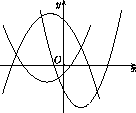
\includegraphics[width=\linewidth]{Сборы/Сборы Элиста 2024/РВ/Algebra/Square_trinomial.png}
\end{wrapfigure}


\problem{3}
На рисунке изображены графики трёх квадратных трёхчленов, нарисованных Джамалом. Может ли Али подобрать такие числа $a, b$ и $c$, чтобы это были графики трёхчленов  $ax^2 + bx + c,  bx^2 + cx + a$  и  $cx^2 + ax + b?$

\problem{4}
Известно, что корни уравнения  $x^2 + px + q = 0$  $-$ целые числа, а $p$ и $q$ $-$ простые числа. Найдите $p$ и $q$.
%https://www.problems.ru/view_problem_details_new.php?id=107740

\problem{5}
Ибрагим написал на доске пять целых чисел $-$ коэффициенты и корни квадратного трёхчлена. Магомед стёр одно из них. Остались числа $2, 3, 4, -5.$ Восстановите стёртое число.
%https://problems.ru/view_problem_details_new.php?id=116690

\problem{6}
Известно, что функция $f(x) = ax^2 + bx + c, \ a \neq 0$ принимает в значения 6, 5 и 5 в трёх последовательных натуральных числах. Найдите наименьшее возможное значение функции $f(x).$

\problem{7}
Даны 2024 квадратных трёхчленов $f_1(x), f_2(x), \ldots , f_{2024}(x)$ таких, что коэффициенты при $x$ и $x^2$ у них совпадают, а вот свободные коэффициенты у всех разные. Известно, что $x_1$ корень $f_1(x)$, $x_2$ корень $f_2(x)$ и т.д. $x_{2024}$ корень $f_{2024}(x)$. Чему равна сумма $f_1(x_2)+f_2(x_3) + \ldots f_{2023}(x_{2024}) + f_{2024}(x_1)$

\problem{8}
Даны квадратные трёхчлены
\[
f_1(x) = x^2 - ax + 2, \quad f_2(x) = x^2 + 3x + b, \quad f_3(x) = 3x^2 + (3 - 2a)x + 4 + b \quad \text{и}\]

$\quad f_4(x) = 3x^2 + (6 - a)x + 2 + 2b.$

Пусть разности их корней равны соответственно \( A, B, C \) и \( D \), и при этом \( |A| \neq |B| \). Найдите соотношение
\[
\frac{C^2 - D^2}{A^2 - B^2}.
\]